\section{Experiments} \label{sec:experiment}

In this section, multiple experiments verify the RRP algorithm with various input parameters. For this an Intel Core i7 2.66 GHz processor with 8GB RAM and running MAC OSX was used. 

Real Yelp Dataset\footnote{https://www.yelp.com/dataset\_challenge} which has both social and spatial components as introduced in the beginning was used. The dataset has 552K social nodes, 77K spatial nodes, 3.5M social edges and 2.2M spatial edges. As social edges indicate friendship strength between users, a random number between 1 to 10 was generated to signify the social distance between two users. Similarly, as every spatial edge is a check-in at a business, the rating given by the user was indicated by a random number between 1 and 10. In both cases larger the number, lower is the friendship strength and lower is the rating respectively. 

The closest vertices returned by {\rrp} are fed into a web application which visualizes the results as shown in Figure \ref{fig:web-app}. The red markers are the places which the user 2AGGIi5EiVLM1XhBXaaAVw visited and flag markers are her recommendations based on social distances. All the recommendations are for the region marked by the translucent black rectangle. The figure also shows the shortest paths listed in ascending order by social distances. Hovering over a node in the path, shows all the information rich attributes that can be used for computing social distance (or edge weights). The details of the application and its source code are available at \url{https://github.com/Nithanaroy/GeoReachRecommender}.

\begin{figure}[t]
	\centering \includegraphics[width=0.40\textwidth]{images/web-app-screenshot.eps}
    \caption{Web Application showing the source vertex, region of interest and the shortest paths}
    \label{fig:web-app}
\end{figure}

Unless specified each run uses the default parameter values as shown in Table \ref{tab:default-param}. Parameter K is the shorthand for top-k, i.e. any query requests 100 closest vertices by default. RZ is the shorthand for resolution which determines the number of blocks the world is divided into. RZ $\gets$ 125 implies that the world is equally into 125 by 125 blocks along latitudes and longitudes. \textit{VertexReachesAlgo} parameter defines how line~\ref{alg:liesin} of algorithm \ref{alg4} is implemented. Throughout this section, it is referred as LIES\_IN. Three implementations which check whether the query region R overlaps with regions reachable from a vertex were used and will be described near those experiments. M and RF are the same parameters described before as the maximum allowed size of a GeoReachSpatial-index entry for a vertex and reduction factor between levels of the GeoReachSpatial-index respectively.

\begin{table}[h]
	\caption{Default parameter values}
	\label{tab:default-param}
	\begin{center}
		\renewcommand{\arraystretch}{1.25}
		\begin{tabular}{ l | l | l }
			\hline
			Parameter & Value & Range \\ \hline
			\hline
			% K & 160 & 10, 20, 40, 80, 160, 320, 640, 1280 \\
			K & 100 & 10, 100, 1000, 10000 \\
			% RZ & 100 & 10, 100, 500, 1000, 5000 \\
			RZ & 125 & 25, 125, 625, 3125 \\
			VertexReachesAlgo & Type 3 & Type 1, Type 2, Type 3 \\
			M & 10K & - \\
			RF & 4 & - \\
			\hline
		\end{tabular}
	\end{center}
\end{table}

\begin{figure}[t]
	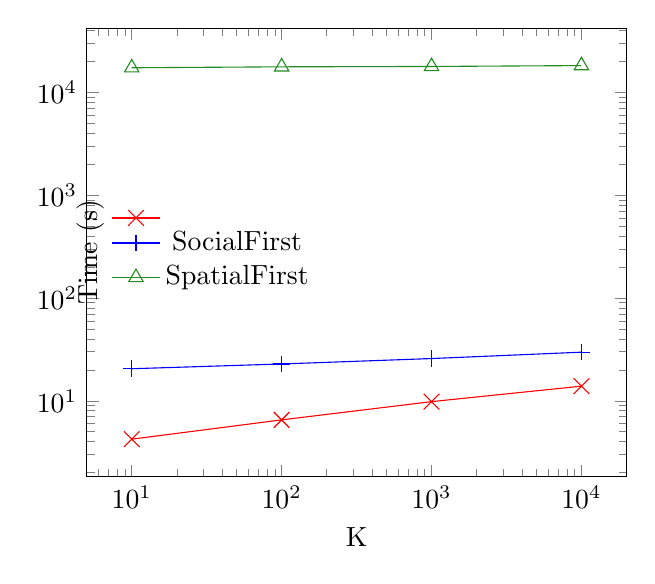
\begin{tikzpicture}[every plot/.append style={}]
	\begin{axis}[
	    xlabel={K},
	    ylabel={Time (s)},
	    xmode = log,
	    ymode = log,
	    legend style={at={(0.03,0.5)},anchor=west},
	    y label style={at={(axis description cs:0.05,.5)}},
		legend style={draw=none},
	    % legend pos=south east,
	    %xmajorgrids=true,
	    %ymajorgrids=true,
	    % xtick={0, 10, 20, 40, 80, 160, 320, 640, 1280},
	    % xticklabel style={rotate=90},
	    %grid style=dashed,
	    % axis line style = ultra thin
	]
	 
	\addplot[
	    color=red,
	    mark=x,
	    mark size=4pt
	    ]
	    coordinates {
	    (10, 4.23)(100, 6.52)(1000, 9.81)(10000, 13.88)
	    %(10, 4.23)(100, 6.52)(500, 9.33)(1000, 9.81)(5000, 13.88)(10000, 13.88)
	    };
	\addplot[
	    color=blue,
	    mark=+,
	    mark size=3pt
	    ]
	    coordinates {
	    (10, 20.5)(100, 22.81)(1000, 25.75)(10000, 29.71)
	    %(10, 20.5)(100, 22.81)(500, 23.04)(1000, 25.75)(5000, 26.61)(10000, 29.71)
	    };
	\addplot[
	    color=ForestGreen,
	    mark=triangle,
	    mark size=3pt
	    ]
	    coordinates {
	    (10, 17382.72)(100, 17755.99)(1000, 17896.76)(10000, 18254.65)
	    };
	    \legend{{\rrp}, SocialFirst, SpatialFirst}
	 
	\end{axis}
	\end{tikzpicture}
	\caption{Runtime comparison among SpatialFirst, SocialFirst and {\rrp} algorithms}
	\label{fig:plot-01}
\end{figure}

{\rrp} is first compared with SocialFirst and SpatialFirst approaches introduced in section \ref{sec:preliminary}. Figure \ref{fig:plot-01} compares the time taken by {\rrp}, SpatialFirst and SocialFirst algorithms for the same source vertex and region. It may seem very intuitive at first that the SpatialFirst algorithm should totally beat others as it is pruning the graph by a huge extent initially using r-tree. To be exact from a graph of 629K nodes, we focused on 2,804 filtered nodes (by r-tree) only which is 0.44\% of the entire graph. Surprisingly, SpatialFirst is 3 orders of magnitude slower than the simple graph traversal SocialFirst algorithm and 4 orders of magnitude slower than {\rrp}. The reason for this massive difference is, A* with landmark is designed for solving single source and single destination problems. In our case A* with landmark function is invoked from the single given source vertex to every destination vertex in the region. Getting into some digits, say A* with landmark takes 3s (which is a very modest number on a real Yelp graph) for computing the shortest path for a given source and destination. Assume the given region R contains 2,000 venues. Therefore A* with landmark is invoked to each of them for a total of 2,000 times, which itself takes about 6,000s or 1.67 hours! Another way to visualize is, the algorithm (from source) is restarted for each of 2,000 destinations which causes it to lose by a huge margin with SocialFirst and {\rrp}.

That is where the SocialFirst algorithm shines. It totally takes a disconnected approach between spatial and social constraints like SpatialFirst, however it doesn't restart for obtaining the next shortest path. SpatialFirst aimlessly wanders the graph in the order of increasing distances from source and emits a result when it finds a vertex in the region. {\rrp} is the best of both the worlds, as it uses a heuristic to traverse the graph in a goal oriented manner towards the region like SpatialFirst and does not restart for obtaining the next shortest destination like SocialFirst. This is the main reason why it shines than the other approaches. And this can be clearly seen in Figure \ref{fig:plot-01}. As SpatialFirst is way out of the league, it is eliminated from the discussion from now on and SocialFirst and {\rrp} are focused. From the plot it is evident that as K increases, the time taken  by {\rrp} and SocialFirst also increases. Though it may be very unlikely that for a query to seek with K $>$ 20, {\rrp} still outperforms SocialFirst algorithm by at least 2 times even in the worst cases. To be specific, the region in the query has 2,804 spatial nodes and K was set as high as 10,000 nodes which is 100\% selectivity for that region and is testing the limits. As the final outcome is clear, the main focus would now be only on {\rrp}. As {\rrp} is made of Spatial Index and Social Index, {\rrp} was run multiple times with and without each index and to study how each of them perform.

\begin{figure*}[t]
	\begin{subfigure}[t]{0.33\textwidth}\centering
		\begin{tikzpicture}[every plot/.append style={}, scale=0.7]
			\begin{axis}[
			    xlabel={K},
			    ylabel={Time (s)},
			    y label style={at={(axis description cs:0.05,.5)}},
			    legend pos=north west,
			    legend style={draw=none},
			    xmode = log,
			    %xmajorgrids=true,
			    %ymajorgrids=true,
			    %grid style=dashed,
			   	mark size=4pt
			]
			 
			%\addplot[
			%    color=blue,
			%    mark=x,
			%    ]
			%    coordinates {
			%    (10,73.8)(20,64.22)(40,64.06)(80,64.66)(160,69.06)(320,69.48)(640,64.44)(1280,64.44)
			%    };
			\addplot[
			    color=blue,
			    mark=triangle,
			    ]
			    coordinates {
			    (10, 9.07)(100, 11.36)(1000, 15.36)(10000, 19.55)
			    %(10, 9.07)(100, 11.36)(500, 13.59)(1000, 15.36)(5000, 19.45)(10000, 19.55)
			    };
			\addplot[
			    color=red,
			    mark=+,
			    ]
			    coordinates {
			    (10, 3.75)(100, 6.04)(1000, 9.81)(10000, 17.65)
			    %(10, 3.75)(100, 6.04)(500, 8.12)(1000, 9.81)(5000, 14.58)(10000, 17.65)
			    };
			\addplot[
			    color=ForestGreen,
			    mark=x,
			    ]
			    coordinates {
			    (10, 4.21)(100, 6.57)(1000, 10.28)(10000, 14.71)
			    %(10, 4.21)(100, 6.57)(500, 8.81)(1000, 10.28)(5000, 13.4)(10000, 14.71)
			    };
			%    \legend{SocialFirst, {\rrpspatial}, {\rrpsocial}, RRP}
			    \legend{{\rrpspatial}, {\rrpsocial}, {\rrp}}
			 
			\end{axis}
		\end{tikzpicture}
		% \caption{Runtime comparison between SocialFirst and types of {\rrp} algorithms for RZ = 10}
		\caption{RZ = 25}
		\label{fig:plot-02}
	\end{subfigure}
	\begin{subfigure}[t]{0.33\textwidth}
		\centering
		\begin{tikzpicture}[every plot/.append style={very thick}, scale=0.7]
			\begin{axis}[
			    xlabel={K},
			    ylabel={Time (s)},
			    y label style={at={(axis description cs:0.05,.5)}},
			    legend pos=north west,
			    legend style={draw=none},
			    xmode = log,
			    %xmajorgrids=true,
			    %ymajorgrids=true,
			    %grid style=dashed,
			    mark size=4pt
			]
			 
			% \addplot[
			%     color=blue,
			%     mark=x,
			%     ]
			%     coordinates {
			%     (10,32.23)(20,29.95)(40,24.9)(80,30.6)(160,24.82)(320,29.76)(640,24.97)(1280,25)
			%     };
			\addplot[
			    color=blue,
			    mark=triangle,
			    ]
			    coordinates {
			    (10, 12.61)(100, 16.01)(1000, 21.12)(10000, 26.04)
			    %(10, 12.61)(100, 16.01)(500, 19.3)(1000, 21.12)(5000, 26.01)(10000, 26.04)
			    };
			\addplot[
			    color=red,
			    mark=+,
			    ]
			    coordinates {
			    (10, 3.79)(100, 6.12)(1000, 9.68)(10000, 21.5)
				%(10, 3.79)(100, 6.12)(500, 8.13)(1000, 9.68)(5000, 19.23)(10000, 21.5)
			    };
			\addplot[
			    color=ForestGreen,
			    mark=x,
			    ]
			    coordinates {
			    (10, 4.97)(100, 7.57)(1000, 11.44)(10000, 18.41)
			    %(10, 4.97)(100, 7.57)(500, 9.86)(1000, 11.44)(5000, 15.81)(10000, 18.41)
			    };
			    % \legend{SocialFirst, {\rrpspatial}, {\rrpsocial}, {\rrp}}
			    \legend{{\rrpspatial}, {\rrpsocial}, {\rrp}}
			 
			\end{axis}
		\end{tikzpicture}
		% \caption{Runtime comparison between SocialFirst and types of {\rrp} algorithms for RZ = 1,000}
		\caption{RZ = 3125}
		\label{fig:plot-03}
	\end{subfigure}
	\begin{subfigure}[t]{0.33\textwidth}
		\centering
		\begin{tikzpicture}[every plot/.append style={very thick}, scale=0.7]
			\begin{axis}[
			    xlabel={K},
			    ylabel={Time (s)},
			    y label style={at={(axis description cs:0.05,.5)}},
			    legend pos=north west,
			    legend style={draw=none},
			    xmode = log,
			    %xmajorgrids=true,
			    %ymajorgrids=true,
			    %grid style=dashed,
			    mark size=4pt
			]
			 
			\addplot[
			    color=blue,
			    mark=triangle,
			    ]
			    coordinates {
			    (10, 9.39)(100, 11.84)(1000, 20.25)(10000, 24.47)
			    %(10, 9.39)(100, 11.84)(500, 14.41)(1000, 20.25)(5000, 22.67)(10000, 24.47)
			    };
			\addplot[
			    color=red,
			    mark=+,
			    ]
			    coordinates {
			    (10, 3.9)(100, 6.0)(1000, 9.67)(10000, 14.58)
			    %(10, 3.9)(100, 6.0)(500, 8.07)(1000, 9.67)(5000, 14.56)(10000, 14.58)
			    };
			\addplot[
			    color=ForestGreen,
			    mark=x,
			    ]
			    coordinates {
			    (10, 3.31)(100, 5.64)(1000, 9.21)(10000, 13.78)
			    %(10, 3.31)(100, 5.64)(500, 7.69)(1000, 9.21)(5000, 13.46)(10000, 13.78)
			    };
			    \legend{{\rrpspatial}, {\rrpsocial}, {\rrp}}
			 
			\end{axis}
		\end{tikzpicture}
		\caption{RZ = 625, lower quality landmark}
		\label{fig:plot-09}
	\end{subfigure}
	\caption{Runtime comparison between the types of {\rrp} algorithms for different resolutions}
\end{figure*}

So the Figure \ref{fig:plot-02} breaks down the components of {\rrp} into {\rrpspatial}, {\rrpsocial} and Both (marked as {\rrp} in the plot's legend). {\rrpspatial} uses only the Spatial index while traversing the graph. As using only {\rrpspatial} index, a heuristic function cannot be built, modified Dijkstra's is used with one extra condition. In Dijkstra's, before adding any vertex to the priority queue, it is verified whether it can reach the given region R using the spatial index. So the sub graphs which cannot reach the region are pruned early using the index. Similarly, {\rrpsocial} uses only the social index for finding the K closest vertices to the source. For this, the algorithm is exactly like algorithm \ref{alg3} except the condition on line~\ref{alg:liesin} of algorithm \ref{alg4} would always return \textbf{false}. This indirectly means spatial index is never used.

Though using either of the indices beat SocialFirst and of course SpatialFirst algorithms, it can be clearly seen that using {\rrpsocial} index outperforms others for smaller K in this case. To understand why it is so, revisit the heuristic algorithm of {\rrp}. The heuristic function uses the Social index with landmark(s). Combined with triangle inequality a lower bound on the distance between the source vertex and a destination vertex in the region is computed. Higher the lower bound, better is the pruning power of {\rrp}. As discussed the quality of landmark(s) plays an important role in the performance. So here using the spatial index only adds the overhead by querying that index, therefore the curve using both the indices slightly underperforms initially. But as K increases, the heuristic’s bound weakens as \textbf{v} in Figure \ref{fig:tri-ine} is no longer small compared to \textbf{u}. At the same time, spatial index helps {\rrp} to make better decisions whenever social index fails. The bottom line, using social index gives better results when:
\begin{itemize}
  \item Quality of the heuristic, indirectly landmarks, is very good
  \item Graph is very dense that most of the vertices can reach the region, making spatial index only an overhead
\end{itemize}

However, as the value of K increases, using both the indices certainly helps as un-necessary graph traversals are further reduced by spatial index. This is clearer in a later experiment when the quality of the landmark is not as good as this case. A very low resolution of 25 by 25 was used above. So how the runtimes change when we increase it by 125 times is studied next.

Just as expected as shown in Figure \ref{fig:plot-03}, the gap between {\rrp} and {\rrpsocial} indices further increases when resolution (RZ) is set to 3125. The function LIES\_IN which checks whether a vertex can reach a region using spatial index takes longer when size of the index entry increases for a given vertex. To totally confirm that this is the case, LIES\_IN was implemented in two more ways which were equivalent w.r.t. runtime but cash on \textit{tiny} advantages based on the size of R and size of spatial index. This is exactly the same parameter VertexReachesAlgo in Table \ref{tab:default-param}. This is how each algorithm is implemented:
\begin{itemize}
  \item \textbf{Type 1}: In this axes transformation technique was used to check if a vertex reaches a region. The axes were transformed such that the southwest corner of the region in the query, is set as origin (0,0). Then for checking if a vertex reaches this region, spatial index entry for the vertex is queried. Then each block number, that the vertex can reach as per spatial index, is transformed into the new co-ordinate system. Then using this transformed 2D block number, a simple comparison of the block with all four corners of the region was used.
  \item \textbf{Type 2}: In this, region (R) in the query is enumerated to block numbers for as many levels as there in the spatial index. Then to check if a vertex reaches this region, each block number from the spatial index for the vertex, are probed with the enumerated region (R). This probing can be done in constant time if blocks reachable by a vertex are stored in a HashSet. This approach performs better than Type 1 if region is really small as the overhead of transforming into a new co-ordinate system is avoided.
  \item \textbf{Type 3}: In this also, region (R) in the query is enumerated to block numbers for all levels in the spatial index. Then a native set intersection function to find if there is match between blocks from R and blocks from a vertex was used. This sometimes shines as native programming implementations which are written in most optimized way especially in higher level languages like Python.
\end{itemize}

\begin{figure*}[t]
	\begin{subfigure}[t]{0.33\textwidth}
		\begin{tikzpicture}[every plot/.append style={thick}, scale=0.70]
			\begin{axis}[
			    xlabel={K},
			    ylabel={Time (s)},
			    legend pos=north west,
			    xmode = log,
			    y label style={at={(axis description cs:0.05,.5)}},
				legend style={draw=none},
			    %xmajorgrids=true,
			    %ymajorgrids=true,
			    %grid style=dashed,
			    mark size=4pt
			]
			 
			% \addplot[
			%     color=blue,
			%     mark=x,
			%     ]
			%     coordinates {
			%     (10,25.67)(20,29.75)(40,25.14)(80,30.61)(160,24.84)(320,24.94)(640,24.95)(1280,24.94)
			%     };
			\addplot[
			    color=blue,
			    mark=triangle,
			    ]
			    coordinates {
			    (10, 9.2)(100, 11.7)(1000, 16.54)(10000, 24.37)
			    %(10, 9.2)(100, 11.7)(500, 13.79)(1000, 16.54)(5000, 19.49)(10000, 24.37)
			    };
			\addplot[
			    color=red,
			    mark=+,
			    ]
			    coordinates {
			    (10, 3.82)(100, 5.97)(1000, 9.6)(10000, 14.52)
				%(10, 3.82)(100, 5.97)(500, 8.02)(1000, 9.6)(5000, 14.5)(10000, 14.52)
			    };
			\addplot[
			    color=ForestGreen,
			    mark=x,
			    ]
			    coordinates {
			    (10, 4.72)(100, 7.23)(1000, 11.04)(10000, 15.74)
			    %(10, 4.72)(100, 7.23)(500, 9.41)(1000, 11.04)(5000, 15.48)(10000, 15.74)
			    };
			    % \legend{SocialFirst, {\rrpspatial}, {\rrpsocial}, {\rrp}}
			    \legend{{\rrpspatial}, {\rrpsocial}, {\rrp}}
			 
			\end{axis}
		\end{tikzpicture}
		\caption{VertexReachAlgo Type 1}
		\label{fig:plot-04}
	\end{subfigure}
	\begin{subfigure}[t]{0.33\textwidth}
		\begin{tikzpicture}[every plot/.append style={thick}, scale=0.70]
			\begin{axis}[
			    xlabel={K},
			    ylabel={Time (s)},
			    legend pos=north west,
			    xmode = log,
			    y label style={at={(axis description cs:0.05,.5)}},
				legend style={draw=none},
			    %xmajorgrids=true,
			    %ymajorgrids=true,
			    %grid style=dashed,
			    mark size=4pt
			]
			 
			% \addplot[
			%     color=blue,
			%     mark=x,
			%     ]
			%     coordinates {
			%     (10,26.11)(20,30.17)(40,25.41)(80,29.98)(160,25.37)(320,24.77)(640,25.03)(1280,24.82)
			%     };
			\addplot[
			    color=blue,
			    mark=triangle,
			    ]
			    coordinates {
			    (10, 9.25)(100, 11.85)(1000, 16.55)(10000, 24.66)
			    %(10, 9.25)(100, 11.85)(500, 13.84)(1000, 16.55)(5000, 19.6)(10000, 24.66)
			    };
			\addplot[
			    color=red,
			    mark=+,
			    ]
			    coordinates {
			    (10, 3.76)(100, 6.01)(1000, 9.68)(10000, 15.24)
				%(10, 3.76)(100, 6.01)(500, 8.14)(1000, 9.68)(5000, 14.71)(10000, 15.24)
			    };
			\addplot[
			    color=ForestGreen,
			    mark=x,
			    ]
			    coordinates {
			    (10, 4.37)(100, 6.74)(1000, 10.42)(10000, 15.42)
			    %(10, 4.37)(100, 6.74)(500, 8.87)(1000, 10.42)(5000, 14.79)(10000, 15.42)
			    };
			    % \legend{SocialFirst, {\rrpspatial}, {\rrpsocial}, {\rrp}}
			    \legend{{\rrpspatial}, {\rrpsocial}, {\rrp}}
			 
			\end{axis}
		\end{tikzpicture}
		% \caption{Runtime comparison between SocialFirst and types of {\rrp} algorithms using VertexReachAlgo Type 2 and RZ = 100}
		\caption{VertexReachAlgo Type 2}
		\label{fig:plot-05}
	\end{subfigure}
	\begin{subfigure}[t]{0.33\textwidth}
		\begin{tikzpicture}[every plot/.append style={thick}, scale=0.70]
			\begin{axis}[
			    xlabel={K},
			    ylabel={Time (s)},
			    legend pos=north west,
			    xmode = log,
			    y label style={at={(axis description cs:0.05,.5)}},
				legend style={draw=none},
			    %xmajorgrids=true,
			    %ymajorgrids=true,
			    %grid style=dashed,
			    mark size=4pt
			]
			 
			% \addplot[
			%     color=blue,
			%     mark=x,
			%     ]
			%     coordinates {
			%     (10,25.14)(20,29.93)(40,25.51)(80,30.6)(160,24.84)(320,24.97)(640,25)(1280,25.09)
			%     };
			\addplot[
			    color=blue,
			    mark=triangle,
			    ]
			    coordinates {
			    (10, 9.36)(100, 11.73)(1000, 16.21)(10000, 24.64)
			    %(10, 9.36)(100, 11.73)(500, 14.41)(1000, 16.21)(5000, 19.95)(10000, 24.64)
			    };
			\addplot[
			    color=red,
			    mark=+,
			    ]
			    coordinates {
			    (10, 3.79)(100, 5.99)(1000, 9.81)(10000, 14.94)
				%(10, 3.79)(100, 5.99)(500, 8.1)(1000, 9.81)(5000, 14.66)(10000, 14.94)
			    };
			\addplot[
			    color=ForestGreen,
			    mark=x,
			    ]
			    coordinates {
			    (10, 4.22)(100, 6.63)(1000, 10.35)(10000, 14.73)
			    %(10, 4.22)(100, 6.63)(500, 8.77)(1000, 10.35)(5000, 14.75)(10000, 14.73)
			    };
			    % \legend{SocialFirst, {\rrpspatial}, {\rrpsocial}, {\rrp}}
			    \legend{{\rrpspatial}, {\rrpsocial}, {\rrp}}
			 
			\end{axis}
		\end{tikzpicture}
		% \caption{Runtime comparison between SocialFirst and types of {\rrp} algorithms using VertexReachAlgo Type 3 and RZ = 100}
		\caption{VertexReachAlgo Type 3}
		\label{fig:plot-06}
	\end{subfigure}
	\caption{Runtime comparison between the types of {\rrp} algorithms for RZ = 625 and various VertexReachAlgo Types}
\end{figure*}

That is how each of the three LIES\_IN algorithms are implemented. Figures \ref{fig:plot-04}, \ref{fig:plot-05}, \ref{fig:plot-06} clearly show that all perform the same way. However, if on mashing the plots together keeping the K constant, Algorithm of Type 3 outperforms in majority of the cases. This confirms the previous doubt that if the resolution is too high like 3125 by 3125 the overhead in LIES\_IN function overcomes the advantage gained by graph pruning in a dense graph. Now to figure out the sweet spot for right value of RZ, experiments comparing K VS Resolution VS Time for each variant of {\rrp} were studied. 

\begin{figure}[t]
	\begin{subfigure}[t]{0.23\textwidth}
		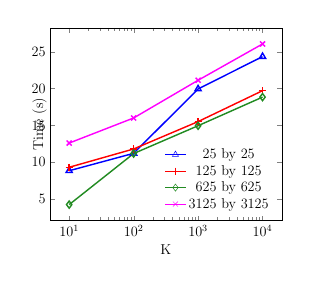
\begin{tikzpicture}[every plot/.append style={very thick}, scale=0.43]
			\begin{axis}[
			    xlabel={K},
			    ylabel={Time (s)},
			    legend pos=south east,
			    xmode = log,
			    %xmajorgrids=true,
			    %ymajorgrids=true,
			    %grid style=dashed,
			    mark size=3pt,
			    xtick=data,
			    % unit vector ratio=1 1 1,
			    % x=0.0015cm,
			    %xticklabels={10, 100, 500, 1000, 5000, 10000}
			    y label style={font=\large, at={(axis description cs:0.005,.5)}},
			    x label style={font=\large},
			    yticklabel style = {font=\large},
			    xticklabel style = {font=\large},
			    legend style={font=\large},
				legend style={draw=none},
			]
			 
			\addplot[
			    color=blue,
			    mark=triangle,
			    ]
			    coordinates {
			    (10, 8.86)(100, 11.22)(1000, 19.94)(10000, 24.33)
			    % (10, 8.86)(100, 11.22)(500, 18.45)(1000, 19.94)(5000, 24.31)(10000, 24.33)
			    %(1, 8.86)(2, 11.22)(3, 18.45)(4, 19.94)(5, 24.31)(6, 24.33)
			    };
			% \addplot[
			%     color=Maroon,
			%     mark=square,
			%     ]
			%     coordinates {
			%     % (10, 4.14)(100, 11.64)(500, 13.52)(1000, 15.1)(5000, 19.33)(10000, 19.31)
			%     (1, 4.14)(2, 11.64)(3, 18.52)(4, 15.1)(5, 19.33)(6, 19.31)
			%     };
			\addplot[
			    color=red,
			    mark=+,
			    ]
			    coordinates {
			    (10, 9.33)(100, 11.81)(1000, 15.52)(10000, 19.71)
				% (10, 9.33)(100, 11.81)(500, 13.82)(1000, 15.52)(5000, 19.66)(10000, 19.71)
				%(1, 9.33)(2, 11.81)(3, 13.82)(4, 15.52)(5, 19.66)(6, 19.71)
			    };
			\addplot[
			    color=ForestGreen,
			    mark=diamond,
			    ]
			    coordinates {
			    (10, 4.27)(100, 11.19)(1000, 14.96)(10000, 18.84)
			    % (10, 4.27)(100, 11.19)(500, 13.4)(1000, 14.96)(5000, 19.02)(10000, 18.84)
			    %(1, 4.27)(2, 11.19)(3, 13.4)(4, 14.96)(5, 19.02)(6, 18.84)
			    };
			\addplot[
			    color=Magenta,
			    mark=x,
			    ]
			    coordinates {
			    (10, 12.61)(100, 16.01)(1000, 21.12)(10000, 26.04)
			    % (10, 12.61)(100, 16.01)(500, 19.3)(1000, 21.12)(5000, 26.01)(10000, 26.04)
			    %(1, 12.61)(2, 16.01)(3, 19.3)(4, 21.12)(5, 26.01)(6, 26.04)
			    };
			    % \legend{5 by 5,25 by 25,125 by 125,625 by 625,3125 by 3125}
			    \legend{25 by 25,125 by 125,625 by 625,3125 by 3125}
			 
			\end{axis}
		\end{tikzpicture}
		\caption{For SpatialIndex of {\rrp}}
		\label{fig:plot-07}
	\end{subfigure}
	\begin{subfigure}[t]{0.23\textwidth}
		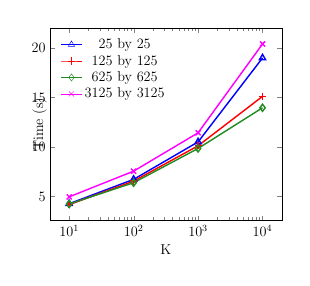
\begin{tikzpicture}[every plot/.append style={very thick}, scale=0.43]
			\begin{axis}[
			    xlabel={K},
			    ylabel={Time (s)},
			    legend pos=north west,
			    xmode = log,
			    %xmajorgrids=true,
			    %ymajorgrids=true,
			    %grid style=dashed,
			    mark size=3pt,
			    xtick=data,
			    %xticklabels={10, 100, 500, 1000, 5000, 10000}
			    y label style={font=\large, at={(axis description cs:0.005,.5)}},
			    x label style={font=\large},
			    yticklabel style = {font=\large},
			    xticklabel style = {font=\large},
			    legend style={font=\large},
				legend style={draw=none},
			]
			 
			\addplot[
			    color=blue,
			    mark=triangle,
			    ]
			    coordinates {
			    (10, 4.28)(100, 6.74)(1000, 10.52)(10000, 19.0)
			    % (10, 4.28)(100, 6.74)(500, 8.92)(1000, 10.52)(5000, 16.09)(10000, 19.0)
			    %(1, 4.28)(2, 6.74)(3, 8.92)(4, 10.52)(5, 16.09)(6, 19.0)
			    };
			% \addplot[
			%     color=Maroon,
			%     mark=square,
			%     ]
			%     coordinates {
			%     % (10, 4.26)(100, 6.67)(500, 8.83)(1000, 10.23)(5000, 14.64)(10000, 14.62)
			%     (1, 4.26)(2, 6.67)(3, 8.83)(4, 10.23)(5, 14.64)(6, 14.62)
			%     };
			\addplot[
			    color=red,
			    mark=+,
			    ]
			    coordinates {
			    (10, 4.19)(100, 6.56)(1000, 10.13)(10000, 15.12)
				% (10, 4.19)(100, 6.56)(500, 8.7)(1000, 10.13)(5000, 14.39)(10000, 15.12)
				%(1, 4.19)(2, 6.56)(3, 8.7)(4, 10.13)(5, 14.39)(6, 15.12)
			    };
			\addplot[
			    color=ForestGreen,
			    mark=diamond,
			    ]
			    coordinates {
			    (10, 4.25)(100, 6.4)(1000, 9.86)(10000, 13.97)
			    % (10, 4.25)(100, 6.4)(500, 8.4)(1000, 9.86)(5000, 13.92)(10000, 13.97)
			    %(1, 4.25)(2, 6.4)(3, 8.4)(4, 9.86)(5, 13.92)(6, 13.97)
			    };
			\addplot[
			    color=Magenta,
			    mark=x,
			    ]
			    coordinates {
			    (10, 4.97)(100, 7.57)(1000, 11.44)(10000, 20.41)
			    % (10, 4.97)(100, 7.57)(500, 9.86)(1000, 11.44)(5000, 16.81)(10000, 20.41)
			    %(1, 4.97)(2, 7.57)(3, 9.86)(4, 11.44)(5, 16.81)(6, 20.41)
			    };
			    % \legend{5 by 5,25 by 25,125 by 125,625 by 625,3125 by 3125}
			    \legend{25 by 25,125 by 125,625 by 625,3125 by 3125}
			 
			\end{axis}
		\end{tikzpicture}
		\caption{For Social+Spatial indices of {\rrp}}
		\label{fig:plot-08}
	\end{subfigure}
	\caption{Runtime comparison between Resolution and K for different types of {\rrp} algorithms}
\end{figure}

From Figure \ref{fig:plot-07} it is evident that as resolution increases for a fixed K and for {\rrpspatial}, performance degrades for very high resolutions due to the overhead by LIES\_IN function. For very low resolutions, as each block is almost the size of Texas, even if a user checks-in at one restaurant there, he/she is considered reachable to that block. So it returns that most vertices can reach R, making it less useful to use a spatial index. The sweet spot so is in between the both extremes, which is 625 in this case. Similar conclusions can be made in next case Figure \ref{fig:plot-08} where both indices were used. But social index lessens the loss brought by spatial index overhead and therefore extreme high resolutions also perform at par with lesser resolutions for smaller K. For larger K even quality of heuristic goes down, so the gap widens.

So after these experiments, it can be concluded that when the graph is really dense using the social index with a high quality landmark is sufficient. Things change when the quality of landmark(s) is not as good. For the next query, the region is even more densely connected and the source vertex is the same, however a lower quality landmark was used. This region has 21,239 spatial nodes which is almost 10 times the count of the previous one.

Figure \ref{fig:plot-09} proves why just having a social index wont help like before. For this region, purposefully a lower quality landmark was chosen. In such cases spatial index prunes majority of the graph as a good resolution of 625 by 625 found earlier was used. Though social index equally performed social+spatial index initially, it lost soon as the landmark quality further degraded for higher K for the same reason explained before. The correctness is never compromised, it is only that {\rrp} tends to Dijkstra's search if landmark quality is not good. Now that when to use each type of index is understood, how each of the algorithms perform with change in region size is studied next.

\begin{figure}[t]
	\begin{subfigure}[t]{0.23\textwidth}
		\begin{tikzpicture}[every plot/.append style={very thick}, scale=0.43]
			\begin{axis}[
			    xlabel={Region Size},
			    ylabel={Time (s)},
			    % legend pos=south west,
			    legend style={at={(0.03,0.5)},anchor=west},
			    % legend style={at={(0,-0.1)},anchor=north},
			    %xmajorgrids=true,
			    %ymajorgrids=true,
			    %grid style=dashed,
			    mark size=4pt,
			    xtick=data,
			    xticklabels={1, 2, 4, 8},
			    y label style={font=\large, at={(axis description cs:0.005,.5)}},
			    x label style={font=\large},
			    yticklabel style = {font=\large},
			    xticklabel style = {font=\large},
			    legend style={font=\large},
				legend style={draw=none},
			]
			 
			% \addplot[
			%     color=blue,
			%     mark=x,
			%     ]
			%     coordinates {
			%     (1, 25.81058407)(2, 30.50130916)(4, 31.07799816)(8, 32.95914412)
			%     };
			\addplot[
			    color=Maroon,
			    mark=x,
			    ]
			    coordinates {
			    (1, 12.77)(2, 10.58)(3, 10.48)(4, 8.42)
			    };
			\addplot[
			    color=red,
			    mark=+,
			    ]
			    coordinates {
			    (1, 4.98)(2, 5.25)(3, 5.24)(4, 5.73)
			    };
			\addplot[
			    color=ForestGreen,
			    mark=triangle,
			    ]
			    coordinates {
			    (1, 4.08)(2, 4.64)(3, 4.59)(4, 5.33)
			    };
			    % \legend{SocialFirst, {\rrpspatial}, {\rrpsocial}, {\rrp}}
			    \legend{{\rrpspatial}, {\rrpsocial}, {\rrp}}
			 
			\end{axis}
		\end{tikzpicture}
		% \caption{Runtime comparison between SocialFirst and types of {\rrp} algorithms for changes in region size for a source vertex S1}
		\caption{For source vertex S1}
		\label{fig:plot-10}
	\end{subfigure}
	\begin{subfigure}[t]{0.23\textwidth}
		\begin{tikzpicture}[every plot/.append style={very thick}, scale=0.43]
			\begin{axis}[
			    xlabel={Region Size},
			    ylabel={Time (s)},
			    legend pos=north east,
			    %xmajorgrids=true,
			    %ymajorgrids=true,
			    %grid style=dashed,
			    mark size=4pt,
			    xtick=data,
			    xticklabels={1, 2, 4, 8},
			    y label style={font=\large, at={(axis description cs:0.005,.5)}},
			    x label style={font=\large},
			    yticklabel style = {font=\large},
			    xticklabel style = {font=\large},
			    legend style={font=\large},
			    x label style={font=\large},
				legend style={draw=none},
			]
			 
			% \addplot[
			%     color=blue,
			%     mark=x,
			%     ]
			%     coordinates {
			%     (1, 26.25)(2, 30.53)(4, 30.52)(8, 32.17)
			%     };
			\addplot[
			    color=Maroon,
			    mark=x,
			    ]
			    coordinates {
			    (1, 12.7)(2, 10.33)(3, 10.35)(4, 8.77)
			    };
			\addplot[
			    color=red,
			    mark=+,
			    ]
			    coordinates {
			    (1, 5.33)(2, 5.42)(3, 5.42)(4, 7.33)
			    };
			\addplot[
			    color=ForestGreen,
			    mark=triangle,
			    ]
			    coordinates {
			    (1, 4.58)(2, 4.64)(3, 4.66)(4, 6.42)
			    };
			    % \legend{SocialFirst, {\rrpspatial}, {\rrpsocial}, {\rrp}}
			    \legend{{\rrpspatial}, {\rrpsocial}, {\rrp}}
			 
			\end{axis}
		\end{tikzpicture}
		% \caption{Runtime comparison between SocialFirst and types of {\rrp} algorithms for changes in region size for a source vertex S2}
		\caption{For source vertex S2}
		\label{fig:plot-11}
	\end{subfigure}
	\caption{Runtime comparison between the types of {\rrp} algorithms VS region size for different source vertices}
	\label{fig:plot1011}
\end{figure}

Figure \ref{fig:plot-10} shows how in every algorithm the time taken linearly increase w.r.t. the size of the region. In Figure \ref{fig:plot1011}, in both the cases users near the source vertex have many check-ins in the given regions and so the spatial index performs worse initially due to its overhead but gradually performs better. The gap further reduces when we a user whose social neighbors do not have many check-ins in the query regions was chosen. Due to this algorithm has to traverse the social graph further down to find the result as shown in Figure \ref{fig:plot-11}.
